\documentclass[
  12pt,
  a4paper,
  oneside
]{article}

% -------------------------------------------------
% Sprache, Kodierung und Schrift
% -------------------------------------------------
\usepackage{iftex}
\ifPDFTeX
  \usepackage[utf8]{inputenc}
  \usepackage[T1]{fontenc}
  \usepackage{lmodern}
\else
  \usepackage{fontspec}
  \setmainfont{lmroman12-regular.otf}[
    BoldFont=lmroman12-bold.otf,
    ItalicFont=lmroman12-italic.otf
  ]
  \setmonofont{lmmono12-regular.otf}
\fi
\usepackage[ngerman]{babel}
\usepackage{microtype}

% -------------------------------------------------
% Seitenlayout
% -------------------------------------------------
\usepackage[
  left=2.5cm,
  right=2.5cm,
  top=2.5cm,
  bottom=2.5cm
]{geometry}
\usepackage{setspace}
\onehalfspacing

% -------------------------------------------------
% Tabellen
% -------------------------------------------------
\usepackage{array}
\usepackage{booktabs}
\usepackage{tabularx}

% -------------------------------------------------
% Mathematische Formeln
% -------------------------------------------------
\usepackage{amsmath}

% -------------------------------------------------
% Literatur und Zitation
% -------------------------------------------------
\usepackage{csquotes}
\usepackage[
  backend=biber,
  style=authoryear,
  sorting=nyt,
  giveninits=true,
  maxcitenames=2,
  maxbibnames=99
]{biblatex}
\addbibresource{literatur.bib}

% -------------------------------------------------
% Abbildungen
% -------------------------------------------------
\usepackage{graphicx}
\usepackage{tikz}
\usetikzlibrary{arrows.meta}

% -------------------------------------------------
% Verweise und Inhaltsverzeichnis
% -------------------------------------------------
\usepackage[
  colorlinks=true,
  linkcolor=black,
  urlcolor=blue,
  citecolor=black
]{hyperref}

\hypersetup{
  pdftitle={Avisierungsservice -- Konzeption und Implementierung},
  pdfauthor={Daniel Tempel}
}

\setcounter{secnumdepth}{3}
\setcounter{tocdepth}{3}

% Unsichtbarer Platzhalter: hält leere Gliederungspunkte umbruchfähig,
% bis der eigentliche Inhalt ergänzt wird.
\newcommand{\contentplaceholder}{%
  \par\noindent\rule{0pt}{\baselineskip}\par
}
\newcommand{\inlinecode}[1]{{\small\texttt{#1}}}

\begin{document}

\tableofcontents
\clearpage

% Die Nummerierung beginnt bei Kapitel 5.
\setcounter{section}{4}

\section{Avisierungsservice -- Konzeption und Implementierung}

Dieses Kapitel beschreibt die Konzeption und technische Umsetzung des
Avisierungsservice. Aufbauend auf der zuvor dargestellten Gesamtarchitektur
werden zunächst die architektonischen, fachlichen und persistenzbezogenen
Grundlagen erläutert. Anschließend werden der Avisierungsprozess, die
Kundenkommunikation, die Mandanten- und
Sicherheitsmechanismen, das Abfragemodell, die Lieferverfolgung und das
Geocoding sowie die technische Konfiguration und lokale Integrationsumgebung
betrachtet. Im Mittelpunkt stehen die Entwurfsentscheidungen, ihre Umsetzung
und ihre Auswirkungen auf Verantwortungsgrenzen, Datenkonsistenz und Betrieb.

\subsection{Architektur-, Domänen- und Persistenzentwurf}
\label{sec:architektur-domaenenentwurf}

\subsubsection{Architekturprinzipien, Verantwortungsgrenzen und Abhängigkeitsrichtung}
\label{sec:architekturprinzipien}

Der Avisierungsservice ist als Java-Anwendung mit Spring Boot umgesetzt, das
als technischer Rahmen des Projekts vorgegeben war. Die Architektur orientiert
sich am Ports-and-Adapters-Ansatz \parencite{cockburn2005hexagonal}.

Die Quellcodeorganisation unterscheidet die Bereiche \texttt{domain},
\texttt{application}, \texttt{adapter} und \texttt{configuration}. Der Domain
Layer enthält die fachlichen Objekte, Zustände und unmittelbar damit
verbundenen Regeln, insbesondere \texttt{Order},
\texttt{ConfirmationRequest} und \texttt{CustomerResponse}. Der Application
Layer koordiniert darauf aufbauend die Anwendungsfälle.

Eingehende Aufrufe werden durch Inbound-Adapter wie REST-Controller oder
Camunda-Delegates entgegengenommen. Ausgewählte ausgehende Integrationen werden
über Outbound-Ports abstrahiert, darunter \texttt{NotificationService} für die
Kundenkommunikation und \texttt{DispoStatusCallbackService} für die
Statusrückmeldung an DISPO. Der Bereich \texttt{configuration} enthält die
Spring-spezifische Konfiguration und Verdrahtung.

Für die portbasiert angebundenen Teile verläuft die statische
Abhängigkeitsrichtung von den Inbound-Adaptern über den Application Layer zum
Domain Layer beziehungsweise vom Application Layer über einen Outbound-Port
zum implementierenden Adapter.

Für den Persistenzzugriff wurde diese Trennung bewusst nicht angewendet. Der
festgelegte Persistenzstack basiert auf Jakarta Persistence (JPA) und Spring
Data JPA. Application-Services greifen daher teilweise direkt auf
Spring-Data-JPA-Repositories und Abstraktionen wie \texttt{Pageable} zu;
zugleich definieren die Domänenklassen ihre relationale Abbildung über
Jakarta-Persistence-Annotationen.

Abbildung~\ref{fig:abhaengigkeitsrichtungen} zeigt die resultierende Adapter-
und Abhängigkeitsstruktur des Avisierungsservice.

% Abbildung unverändert

Auf separate Repository-Ports, Persistence-Entities und die damit verbundene
Mappinglogik wurde verzichtet. Eine Austauschbarkeit der Persistenztechnologie
war im Projektumfang nicht gefordert und hätte zusätzlichen Struktur- und
Mappingaufwand verursacht.

Diese Entscheidung koppelt den Application Layer stärker an Spring Data und
das Domänenmodell an Jakarta Persistence. Änderungen des Persistenzstacks oder
seiner Mappinganforderungen können daher Anpassungen in diesen Bereichen
erfordern.

Die Umsetzung entspricht somit keiner strikt technologieunabhängigen
hexagonalen Architektur, sondern kombiniert die portbasierte Entkopplung
ausgewählter Integrationen mit der direkten Einbindung des festgelegten
Persistenzstacks.

\subsubsection{Domänen- und Zustandsmodell}
\label{sec:domaenenmodell}

Das Domänenmodell trennt den aus DISPO übernommenen Auftrag, einzelne
Rückbestätigungsanfragen und die darauf bezogenen Kundenreaktionen. Fachliche,
technische und prozessbezogene Zustände werden jeweils dem Objekt zugeordnet,
dessen Verantwortung sie beschreiben.

\texttt{Company} bildet den Mandantenbezug. Jeder \texttt{Order} ist genau
einer \texttt{Company} zugeordnet; auch die externe Auftragsidentität wird in
diesem Mandantenkontext betrachtet. Die technische Mandantentrennung wird in
Abschnitt~\ref{sec:mandantenkontext} behandelt.

\texttt{Order} repräsentiert den aus DISPO übernommenen fachlichen Auftrag mit
den für die Avisierung relevanten Auftrags- und Tourdaten. Sein
\texttt{confirmationStatus} beschreibt den auftragsbezogenen Stand des
Avisierungsprozesses.

Eine konkrete Avisierung wird durch \texttt{ConfirmationRequest} abgebildet.
Sie enthält unter anderem Token, Kommunikationskanal, Lieferfenster und
Antwortfrist. Ein \texttt{Order} kann mehrere aufeinanderfolgende
\texttt{ConfirmationRequest}-Objekte besitzen, sodass frühere Anfragen als
Avisierungshistorie erhalten bleiben.

Der \texttt{deliveryStatus} eines \texttt{ConfirmationRequest} beschreibt den
technischen Versandstand. \texttt{SENT} bedeutet lediglich, dass der
Versandaufruf ohne gemeldeten technischen Fehler abgeschlossen wurde; eine
tatsächliche Zustellung oder Kenntnisnahme des Kunden wird dadurch nicht
nachgewiesen.

Das zusätzliche Merkmal \texttt{active} kennzeichnet unabhängig vom
Versandstatus, ob die Anfrage noch als gültige Grundlage für eine
Kundenreaktion dient. Die konkreten Zustandsübergänge werden in
Abschnitt~\ref{sec:prozessumsetzung} beschrieben.

Eine \texttt{CustomerResponse} ist genau derjenigen
\texttt{ConfirmationRequest} zugeordnet, auf die sich die Kundenentscheidung
bezieht. Dadurch bleibt nachvollziehbar, auf welches Lieferfenster der Kunde
reagiert hat. Pro Anfrage kann höchstens eine Kundenreaktion gespeichert
werden; zusätzlich können ein Kommentar und der Eingangszeitpunkt
\texttt{receivedAt} erfasst werden.

Die eingebetteten Fachstrukturen \texttt{Tour} und \texttt{DeliverySlot}
besitzen keinen eigenständigen Lebenszyklus. \texttt{Tour} umfasst Tournummer
und Fahrzeugkennzeichen. \texttt{DeliverySlot} repräsentiert Datum, Beginn und
Ende des vorgeschlagenen Lieferfensters und stellt sicher, dass dessen Beginn
vor dem Ende liegt.

\texttt{CompanyEmailSettings} enthält die mandantenspezifische
E-Mail-Konfiguration und ist höchstens einmal einer \texttt{Company}
zugeordnet. Die technische Ausgestaltung wird in
Abschnitt~\ref{sec:emailversand}, der Schutz sensibler Werte in
Abschnitt~\ref{sec:konfigurationsschutz} behandelt.

Tabelle~\ref{tab:zustandsdimensionen} fasst die getrennt modellierten
Zustandsaspekte zusammen.

% Tabelle unverändert

Die Trennung verhindert eine Vermischung fachlicher und technischer Zustände.
Ein fehlgeschlagener Versand stellt beispielsweise keine Ablehnung des Kunden
dar; ebenso bedeutet ein technisch erfolgreicher Versand noch keine
Bestätigung des vorgeschlagenen Liefertermins.

\subsubsection{Persistenzmodell und Schemaentwicklung}
\label{sec:persistenzmodell}

Das Persistenzmodell basiert auf PostgreSQL. Die relationale Abbildung erfolgt
über Jakarta Persistence mit Hibernate als Persistence Provider; für den
Datenzugriff wird Spring Data JPA eingesetzt. Wie in
Abschnitt~\ref{sec:architekturprinzipien} beschrieben, befinden sich die
JPA-Mappings unmittelbar in den Domänenklassen.

\texttt{Company}, \texttt{Order}, \texttt{ConfirmationRequest} und
\texttt{CustomerResponse} werden in den Tabellen \texttt{company},
\texttt{order\_snapshot}, \texttt{confirmation\_request} und
\texttt{customer\_response} persistiert. Die mandantenspezifische
E-Mail-Konfiguration liegt in \texttt{company\_email\_settings}.

Die eingebetteten Strukturen \texttt{Tour} und \texttt{DeliverySlot} besitzen
keine eigenen Tabellen. Tournummer und Fahrzeugkennzeichen werden in
\texttt{order\_snapshot} gespeichert; Datum sowie Beginn und Ende des
Lieferfensters in \texttt{confirmation\_request}.

Abbildung~\ref{fig:persistenzmodell} zeigt die zentralen anwendungseigenen
Tabellen, ihre Beziehungen sowie ausgewählte Schlüssel- und
Eindeutigkeitsbedingungen. Von Camunda und Flyway verwaltete technische
Tabellen werden nicht dargestellt.

% Abbildung unverändert

Die Zuordnung eines \texttt{Order} zu seiner \texttt{Company} erfolgt über
\texttt{company\_id}. Da die aus DISPO übernommene
\texttt{external\_order\_id} nur innerhalb eines Mandanten eindeutig sein muss,
ist die Kombination aus \texttt{company\_id} und
\texttt{external\_order\_id} eindeutig definiert.

Ein \texttt{ConfirmationRequest} verweist über
\texttt{order\_snapshot\_id} auf den zugehörigen Auftrag. Sein Token ist
schemaweit eindeutig; ob er für einen Kundenzugriff noch gültig ist, entscheidet
davon unabhängig die Anwendungslogik. Die Eindeutigkeit von
\texttt{customer\_response.confirmation\_request\_id} begrenzt jede Anfrage
auf höchstens eine Kundenreaktion. Analog stellt die Eindeutigkeit von
\texttt{company\_email\_settings.company\_id} höchstens einen
E-Mail-Konfigurationsdatensatz pro Mandant sicher.

Zusätzliche \texttt{CHECK}-Constraints sichern ausgewählte strukturelle
Gültigkeitsregeln ab. So muss \texttt{response\_deadline\_hours} positiv sein;
für die E-Mail-Konfiguration bestehen unter anderem Bedingungen für SMTP-Port
und erforderliche Zugangsdaten bei aktivierter Authentifizierung.

Nicht alle fachlichen Invarianten werden zusätzlich in der Datenbank
abgebildet. Die Reihenfolge von Beginn und Ende eines \texttt{DeliverySlot}
wird beispielsweise im Domänenmodell geprüft. Die Datenbank sichert damit
insbesondere referenzielle Integrität, Eindeutigkeit und ausgewählte
strukturelle Wertebereiche.

Ergänzende Indizes unterstützen insbesondere mandanten- und tourbezogene
Abfragen sowie den Zugriff auf die Rückbestätigungsanfragen eines Auftrags.

Die Schemaentwicklung wird mit Flyway gesteuert. Änderungen werden als
versionierte Migrationen in definierter Reihenfolge ausgeführt und in der
Flyway-Schemahistorie dokumentiert, wodurch sie reproduzierbar auf
unterschiedliche Laufzeitumgebungen übertragen werden können
\parencite{redgate2024versionedMigrations}. Hibernate ist mit
\texttt{ddl-auto: validate} konfiguriert und verändert das Schema nicht selbst,
sondern prüft beim Anwendungsstart dessen Kompatibilität mit den JPA-Mappings.

Ausgewählte Migrationen zeigen die Weiterentwicklung des Persistenzmodells.
Mit \texttt{V6} wurde die Mandantenfähigkeit eingeführt: Die Tabelle
\texttt{company} und \texttt{company\_id} in \texttt{order\_snapshot} wurden
ergänzt und die zuvor globale Eindeutigkeit der
\texttt{external\_order\_id} durch die mandantenbezogene Eindeutigkeit von
\texttt{company\_id} und \texttt{external\_order\_id} ersetzt.

Mit \texttt{V9} wurde \texttt{company\_email\_settings} für die
mandantenspezifische E-Mail-Konfiguration ergänzt. \texttt{V10} führte den
technischen \texttt{delivery\_status} in
\texttt{confirmation\_request} ein und bildete damit die technische
Versandverarbeitung als eigenen Zustand auch im Persistenzmodell ab.

Das Persistenzmodell überträgt damit die zentralen Beziehungen des
Domänenmodells und ausgewählte Integritätsregeln in die relationale
Datenstruktur; seine Weiterentwicklung erfolgt kontrolliert über Flyway.

\subsection{Technische Umsetzung des Avisierungsprozesses}
\label{sec:prozessumsetzung}

Der Avisierungsprozess umfasst die Übernahme des Avisierungsauftrags aus DISPO,
die Benachrichtigung des Kunden, die Verarbeitung der Rückbestätigung oder eines
Fristablaufs sowie die abschließende Statusrückmeldung an DISPO. Er verbindet
damit die synchrone Auftragsübernahme mit einer nachgelagerten, zeitlich
verteilten Verarbeitung. Die folgenden Abschnitte beschreiben diesen
technischen Lebenszyklus bis zur Behandlung von Fehlern, Wiederholungen und
Nebenläufigkeit.

\subsubsection{Übernahme von Avisierungsaufträgen, Validierung und Prozessstart}
\label{sec:auftragsuebernahme}

Ein Avisierungsauftrag wird über eine REST-Schnittstelle aus DISPO übernommen
und zusammen mit dem bereits bestimmten Mandantenkontext an die
Anwendungslogik übergeben. Ob dabei eine neue Rückbestätigungsanfrage und
Prozessinstanz entstehen, hängt vom vorhandenen Verarbeitungszustand ab. Die
vorgelagerte Authentifizierung und Ermittlung des Mandantenkontexts werden in
Abschnitt~\ref{sec:dispo-authentifizierung} beschrieben.

Der Auftrag enthält die für die Avisierung erforderlichen Auftrags-, Tour-,
Kunden-, Kontakt- und Lieferdaten sowie Prozessparameter wie
Kommunikationskanal und Antwortfrist.

Die Eingangsdaten werden zunächst an der Schnittstellengrenze strukturell
validiert. Dazu gehören Pflichtfelder, Formatvorgaben und Wertebereiche.
Fachlich kontextabhängige Regeln werden anschließend in der Anwendungslogik
beziehungsweise im Domänenmodell geprüft. So muss für den gewählten
Kommunikationskanal die passende Kontaktinformation vorliegen, und das
übermittelte Lieferfenster darf zum Zeitpunkt der Auftragsübernahme noch nicht
begonnen haben. Dadurch werden strukturelle und fachliche Validierung getrennt,
bevor eine neue Prozessverarbeitung initialisiert wird.

Der Mandantenkontext bestimmt den zu verwendenden Datenbestand. Die zugehörige
\texttt{Company} wird daraus ermittelt; ein bestehender \texttt{Order} wird
über Mandanten-ID und externe Auftrags-ID gesucht. Eine erneut übertragene
externe Auftrags-ID führt daher nicht automatisch zu einem weiteren
\texttt{Order}-Objekt.

Die weitere Verarbeitung ist zustandsabhängig. Der Avisierungsservice
berücksichtigt den bestehenden \texttt{Order} und dessen letzte
Rückbestätigungsanfrage und vergleicht deren relevante Daten mit dem neu
eingegangenen Auftrag. Daraus ergibt sich, ob die bestehende Verarbeitung
weiterverwendet oder aktualisiert werden kann oder eine neue
Rückbestätigungsanfrage mit neuer Prozessinstanz erforderlich ist.
Tabelle~\ref{tab:avisierungsauftrag-entscheidung} fasst diese Entscheidung
zusammen.

% Tabelle unverändert

Eine identische erneute Übertragung erzeugt bei einer bereits laufenden
\texttt{PENDING}-Anfrage keine zusätzliche Prozessinstanz. Ändern sich die
Daten in diesem Zustand, werden Auftrag und bestehende Anfrage aktualisiert,
wodurch ihre Zuordnung zur vorhandenen Prozessinstanz erhalten bleibt. Auch
eine aktive \texttt{SENT}-Anfrage oder ein weiterhin verwendbares
abgeschlossenes Ergebnis kann bei unveränderten Daten wiederverwendet werden.

Ist eine neue Rückbestätigungsanfrage erforderlich, wird ein Token für den
späteren Kundenzugriff erzeugt und ein neuer \texttt{ConfirmationRequest} mit
Kommunikationskanal, Lieferfenster und Antwortfrist im Versandstatus
\texttt{PENDING} gespeichert. Zu diesem Zeitpunkt ist die Anfrage noch nicht
für Kundenreaktionen aktiviert. Die nach der Persistierung verfügbare interne
ID dient zur Zuordnung und zum Start der Prozessinstanz; der davon unabhängige
Token wird ausschließlich für den Kundenzugriff verwendet
(vgl. Abschnitt~\ref{sec:kundenzugriff-token}).

Der Prozessstart erfolgt noch innerhalb der Auftragsübernahme, der eigentliche
Nachrichtenversand jedoch erst nach einer asynchronen Fortsetzungsstelle. Der
HTTP-Aufruf bestätigt somit die Übernahme des Auftrags, während die von
externen Kommunikationssystemen abhängige Verarbeitung nachgelagert durch die
Workflow Engine ausgeführt wird.

Dies spiegelt sich in der HTTP-Semantik wider. Befindet sich der Auftrag nach
der Verarbeitung weiterhin im Status \texttt{OPEN}, antwortet die
DISPO-Schnittstelle mit \texttt{202 Accepted}. Dies bedeutet weder, dass die
Nachricht bereits versendet wurde, noch zwingend, dass eine neue
Prozessinstanz entstanden ist. Ein bereits vorhandener und weiterhin
verwendbarer Zustand führt dagegen zu \texttt{200 OK}; dies umfasst sowohl
eine aktive \texttt{SENT}-Anfrage als auch die Ergebnisse
\texttt{CONFIRMED} oder \texttt{REJECTED}.

Die Auftragsübernahme trennt damit strukturelle und fachliche Validierung,
ordnet den Auftrag einem Mandanten zu und entscheidet zustandsabhängig über
Wiederverwendung, Aktualisierung oder Neuerzeugung der weiteren Verarbeitung.

Fehler an den REST-Schnittstellen werden zentral in ein einheitliches
Fehlerformat überführt. Strukturelle Validierungsfehler, fachliche Konflikte und
technische Fehler werden dabei unterschiedlichen HTTP-Statuscodes und
Fehlerkennungen zugeordnet. Dadurch bleibt die Fehlerbehandlung der Controller
von den einzelnen Ausnahmearten getrennt, und die Schnittstellen liefern ein
konsistentes Fehlerformat.

\subsubsection{Dauerhafte Workflow-Steuerung mit Camunda}
\label{sec:workflow-steuerung}

Der Avisierungsprozess umfasst Wartezeiten und Ereignisse, die unabhängig
vom ursprünglichen HTTP-Aufruf eintreten. Nach dem Versand wartet er
beispielsweise auf eine Kundenreaktion, den Ablauf der Antwortfrist oder die
Ablösung durch eine neuere Avisierung. Diese Anforderungen erfordern dauerhaft
persistierbare Wartezustände sowie zeit- und ereignisabhängige Fortsetzungen.

Dafür wurde eine workflowbasierte Prozesssteuerung gewählt. Eine rein
anwendungsseitige Lösung hätte Wartezustände, Timer und Ereigniskorrelation
zusätzlich in Anwendungslogik und Persistenz abbilden müssen. Eine Workflow
Engine ermöglicht dagegen ein ausführbares Prozessmodell und übernimmt dessen
Ablaufkoordination. Dem stehen eine zusätzliche Laufzeitkomponente, höherer
Integrations- und Betriebsaufwand sowie eine teilweise Bindung an
enginespezifische Schnittstellen gegenüber.

Als konkrete Workflow Engine wird Camunda 7 eingesetzt. Sie übernimmt die
Ausführung der BPMN-Prozessdefinition, persistente Wartezustände, Timer,
Nachrichtenkorrelation und die Anbindung von Service Tasks an Java-Code. Die
Workflow Engine ist in die Spring-Boot-Anwendung integriert; die BPMN-Modelle
werden beim Start automatisch deployt. Die Runtime API wird unter anderem für
Prozessstarts und Nachrichtenkorrelation verwendet
\parencite{camunda724processEngineConcepts}.

Während Kapitel 3 den fachlichen SOLL-Prozess beschreibt, zeigt
Abbildung~\ref{fig:confirmation-request-process} dessen technische
Konkretisierung durch Service Tasks, Wartezustände, Nachrichtenereignisse,
Timer und Fehlerpfade.

% Abbildung unverändert

Das BPMN-Modell wird unter dem Schlüssel
\texttt{confirmation-request-process} deployt. Jede Prozessinstanz repräsentiert
einen konkreten Avisierungsvorgang und ist über die interne
\texttt{ConfirmationRequest.id} als Business Key einer
Rückbestätigungsanfrage zugeordnet. Derselbe Schlüssel wird zusammen mit dem
jeweiligen Message-Namen zur Korrelation von Kundenreaktionen oder
Ablösungsereignissen verwendet.

Der fachliche Zustand verbleibt in den Domänenobjekten und der
Anwendungsdatenbank. Die Workflow Engine verwaltet dagegen den
Ausführungszustand der Prozessinstanz und die für die Ablaufsteuerung
erforderlichen Prozessvariablen. Sie ergänzt somit das fachliche Datenmodell um
den für die Orchestrierung notwendigen Prozesszustand.

Die Integration erfolgt in beide Richtungen.
Tabelle~\ref{tab:workflow-integration} fasst die technischen Bindeglieder und
Verantwortlichkeiten zusammen.

% Tabelle unverändert

Java Delegates bilden die Camunda-spezifische Schnittstelle zur
Anwendungslogik. Sie lesen Business Key und Prozessvariablen, rufen die
zugehörigen Use Cases auf und überführen deren Ergebnisse in den
BPMN-Ablauf. Beim Versand kann das Ergebnis beispielsweise über
Prozessvariablen weitergegeben oder als \texttt{BpmnError} an ein Boundary
Error Event signalisiert werden. Die fachliche Verarbeitung verbleibt damit im
Application Layer.

Die Trennung vom ursprünglichen HTTP-Aufruf wird durch eine asynchrone
Fortsetzungsstelle vor dem Nachrichtenversand umgesetzt. Der Prozessstart
erfolgt noch synchron, die weitere Verarbeitung anschließend als Job der
Workflow Engine.

Nach erfolgreichem Versand erreicht die Prozessinstanz ein ereignisbasiertes
Gateway und wartet dort auf Kundenreaktion, Fristablauf oder Ablösung. Dabei
bleibt kein Anwendungsthread blockiert; die Instanz wird erst durch das
eintretende Ereignis fortgesetzt.

Für fehlgeschlagenen Nachrichtenversand enthält das BPMN-Modell einen eigenen
Fehlerpfad. Die konkrete Fehlerklassifikation und Wiederholungsstrategie werden
in Abschnitt~\ref{sec:fehlerbehandlung} beschrieben.

Damit verbleibt die fachliche Zustandsführung im Avisierungsservice, während
die Workflow Engine die zeit- und ereignisabhängige Ablaufkoordination
übernimmt.

\subsubsection{Kundenreaktion und Fristablauf}
\label{sec:kundenreaktion-fristablauf}

Bevor eine Kundenreaktion übermittelt wird, stellt der Avisierungsservice die
für die Bestätigungsseite benötigten Auftrags- und Lieferinformationen anhand
des im Bestätigungslink enthaltenen Tokens bereit. Dabei wird ausschließlich
die jeweils neueste Rückbestätigungsanfrage eines Auftrags berücksichtigt.
Neben den Lieferdaten wird aus dem Zustand der Anfrage und einer gegebenenfalls
bereits vorhandenen Kundenreaktion der darzustellende Bestätigungsstatus
abgeleitet.

Nach einem technisch erfolgreichen Versand wird die Rückbestätigungsanfrage in
den Versandstatus \texttt{SENT} überführt, \texttt{sentAt} gespeichert und mit
\texttt{active = true} für Kundenreaktionen aktiviert. Gleichzeitig wechselt
der zugehörige \texttt{Order} von \texttt{OPEN} nach \texttt{SENT}.

Mit dem Versand wird der tatsächliche Ablaufzeitpunkt bestimmt. Er entspricht
dem früheren Zeitpunkt aus konfigurierter Antwortdauer ab
\texttt{sentAt} und Beginn des Lieferfensters:

\[
\begin{aligned}
	\texttt{expiresAt}
	= \min\!\bigl(
	&\texttt{sentAt} + \text{konfigurierte Antwortdauer}, \\
	&\text{Beginn des Lieferfensters}
	\bigr)
\end{aligned}
\]

Die Antwortdauer wird über \texttt{responseDeadlineHours} angegeben. Dadurch
beginnt die Frist erst nach erfolgreichem Versand und endet spätestens mit dem
Beginn des Lieferfensters.

Kundenreaktionen werden über den in der Nachricht enthaltenen Token
entgegengenommen. Dieser muss zur jeweils neuesten
\texttt{ConfirmationRequest} des Auftrags gehören, sodass überholte Anfragen
nicht mehr beantwortet werden können. Die sicherheitsbezogene Ausgestaltung
wird in Abschnitt~\ref{sec:kundenzugriff-token} beschrieben.

Der Kunde kann den Liefertermin mit \texttt{CONFIRM} bestätigen oder mit
\texttt{REJECT} ablehnen und optional einen Kommentar übermitteln. Vor der
Verarbeitung wird geprüft, ob die Anfrage weiterhin aktiv, noch nicht
abgelaufen und unbeantwortet ist. Eine Antwort ist nur zulässig, solange
\texttt{receivedAt}~$<$~\texttt{expiresAt} gilt.

Bei einer gültigen Antwort wird der \texttt{Order} auf
\texttt{CONFIRMED} beziehungsweise \texttt{REJECTED} gesetzt, die
\texttt{CustomerResponse} gespeichert und die Anfrage deaktiviert. Ihr
technischer Versandstatus bleibt \texttt{SENT}, da die Kundenentscheidung den
bereits erfolgten Versand nicht verändert.

Anschließend wird die Kundenreaktion mit der Prozessinstanz korreliert. Eine
zusätzliche Eingangsbestätigung an den Kunden wird als nachgelagerter
Kommunikationseffekt ausgelöst. Schlägt dieser Versand fehl, wird der Fehler
protokolliert; die bereits gespeicherte Kundenentscheidung bleibt bestehen.

Der alternative Pfad ist der Fristablauf über das im Workflow hinterlegte
Timer-Ereignis. Vor einer fachlichen Zustandsänderung prüft die
Anwendungslogik erneut, ob die Anfrage noch aktiv und
\texttt{expiresAt} tatsächlich erreicht ist. Nur dann wird sie deaktiviert und
der \texttt{Order} auf \texttt{NO\_RESPONSE} gesetzt. Der
\texttt{deliveryStatus} bleibt auch hier \texttt{SENT}.

Das Ausbleiben einer Antwort ist damit kein Versandfehler, sondern das
fachliche Ergebnis einer zuvor erfolgreich eröffneten Antwortphase. Der Timer
bildet lediglich den technischen Auslöser; die Zulässigkeit des
Zustandsübergangs entscheidet weiterhin die Anwendungslogik.

Tabelle~\ref{tab:kundenreaktion-fristablauf} fasst die resultierenden
Zustandsübergänge zusammen.

% Tabelle unverändert

Eine gültige Kundenentscheidung oder der Fristablauf beendet die aktive
Antwortphase. Der Auftrag befindet sich anschließend in
\texttt{CONFIRMED}, \texttt{REJECTED} oder \texttt{NO\_RESPONSE}; die Anfrage
ist deaktiviert und behält ihren technischen Versandstatus \texttt{SENT}.
Daneben kann eine laufende Anfrage durch eine neuere Avisierung abgelöst
werden.

\subsubsection{Erneute Avisierung und Ablösung veralteter Anfragen}
\label{sec:erneute-avisierung}

Eine erneute Verarbeitung kann auf zwei Wegen ausgelöst werden. Einerseits kann
DISPO einen bereits bekannten Auftrag erneut übermitteln, beispielsweise
aufgrund geänderter Auftrags- oder Avisierungsdaten oder nach einem zuvor
erfolglosen Avisierungsversuch. Andererseits kann nach einem endgültigen
Zustellfehler oder einem Fristablauf ohne Kundenreaktion eine erneute Avisierung
manuell über das Avisierungsdashboard angestoßen werden. Beide Wege können zur
Erzeugung einer neuen Rückbestätigungsanfrage führen, unterscheiden sich jedoch
hinsichtlich ihrer Änderungsmöglichkeiten und fachlichen Voraussetzungen.

Sind bei der erneuten Übermittlung durch DISPO die Daten einer bereits
versendeten Anfrage geändert, kann die bisherige Anfrage nicht weiterverwendet
werden. Eine noch aktive Anfrage wird daher deaktiviert und die zugehörige
wartende Prozessinstanz über das Ereignis
\texttt{ConfirmationRequestSuperseded} beendet. Die abgelöste Prozessinstanz
endet auf diesem Pfad ohne fachliche Statusrückmeldung an DISPO. Maßgeblich für
die weitere Verarbeitung ist anschließend die neu erzeugte
Rückbestätigungsanfrage.

Wird aufgrund des bestehenden Zustands eine neue Rückbestätigungsanfrage
erzeugt, werden deren anfragespezifische Daten separat gespeichert. Dadurch
bleiben das jeweilige Lieferfenster, der Kommunikationskanal, die Antwortfrist
und der Versandstatus der einzelnen Versuche nachvollziehbar.

\subsubsection{Statusrückmeldung an DISPO}
\label{sec:statusrueckmeldung-dispo}

Beim Abschluss des ursprünglichen HTTP-Aufrufs aus DISPO liegt noch
kein Rückbestätigungsergebnis vor. Eine Kundenentscheidung kann unmittelbar
nach dem Versand, aber auch erst nach längerer Wartezeit eintreten; alternativ
kann die Antwortfrist ohne Kundenreaktion ablaufen. Das Integrationskonzept
sieht daher einen mandantenspezifisch konfigurierten Callback-Endpunkt vor, über
den der Avisierungsservice den später feststehenden Status an DISPO
zurückmeldet.

Die Statusrückmeldung ist Bestandteil des regulären Prozesspfads und erfolgt
vor dessen Abschluss. Das ausführbare Prozessmodell führt die Zustände
\texttt{CONFIRMED}, \texttt{REJECTED} und \texttt{NO\_RESPONSE} zu diesem
Schritt. Ein technischer Zustellfehler mit dem Versandstatus \texttt{FAILED}
sowie die Ablösung einer Rückbestätigungsanfrage durch eine neuere Avisierung
enden dagegen auf separaten Prozesspfaden. Der Callback-Schritt übergibt den
bereits bestimmten Status zusammen mit der Identität der zugrunde liegenden
Rückbestätigungsanfrage an die Anwendungslogik zur externen Rückmeldung.

Vor dem HTTP-Aufruf wird geprüft, ob die zugrunde liegende
Rückbestätigungsanfrage noch aktuell ist. Hierzu wird die jüngste
\texttt{ConfirmationRequest} des betreffenden \texttt{Order} bestimmt und ihre
ID mit der im Business Key der Prozessinstanz enthaltenen Anfrage-ID
verglichen. Nur bei Übereinstimmung wird die Rückmeldung ausgeführt.

Diese Prüfung verhindert insbesondere die Übertragung eines bereits überholten
Status. Wird beispielsweise nach einer Rückbestätigungsanfrage A aufgrund
geänderter Avisierungsdaten eine neue Anfrage B erzeugt und erreicht die
Prozessinstanz von A erst danach den Callback-Schritt, wird die Rückmeldung von
A unterdrückt. Anfrage A ist zu diesem Zeitpunkt nicht mehr die jüngste
Rückbestätigungsanfrage des Auftrags.

Ist die Anfrage weiterhin aktuell, wird das Callback-Ziel aus der dem Auftrag
zugeordneten \texttt{Company} bestimmt. Dadurch kann für jeden Mandanten ein
eigener DISPO-Endpunkt konfiguriert werden. Übertragen werden die externe
Auftrags-ID, der Rückbestätigungsstatus und, sofern vorhanden, ein vom Kunden
übermittelter Kommentar. Die ursprünglich aus DISPO übernommene externe
Auftrags-ID ermöglicht die Zuordnung zur dortigen Auftragsidentität, ohne dass
interne Datenbankidentifikatoren des Avisierungsservice über die Systemgrenze
übertragen werden.

Wird die Rückmeldung aufgrund einer inzwischen neueren Anfrage unterdrückt,
endet der Prozesspfad regulär ohne externen HTTP-Aufruf. Nach erfolgreicher
Statusübertragung erreicht die Prozessinstanz ebenfalls ihr abschließendes
Endereignis.

\subsubsection{Fehlerbehandlung, Wiederholungen, Nebenläufigkeit und Idempotenzgrenzen}
\label{sec:fehlerbehandlung}

Neben dem regulären Prozessablauf muss der Avisierungsservice auch
fehlgeschlagene, wiederholte und gleichzeitig ausgeführte Verarbeitungsschritte
berücksichtigen. Hierfür werden unterschiedliche Mechanismen eingesetzt:
Wiederholungen innerhalb des Workflows, technische Wiederholungsversuche durch
die Workflow Engine, Datenbanksperren sowie Prüfungen des bereits erreichten
Zustands.

Beim Nachrichtenversand werden Fehler danach unterschieden, ob ein weiterer
Versandversuch sinnvoll vorgesehen ist oder der Versand unmittelbar als
fehlgeschlagen behandelt wird. Vom Kommunikationssystem gemeldete
Zustellfehler werden grundsätzlich als wiederholbar behandelt. Eine feinere
Unterscheidung zwischen kurzfristigen und dauerhaft bestehenden Ursachen
erfolgt dabei nicht. Nicht wiederholbar sind dagegen beispielsweise eine
fehlende notwendige E-Mail-Konfiguration oder der Fall, dass ein bei der
Auftragsübernahme noch gültiges Lieferfenster zum tatsächlichen Versandzeitpunkt
bereits begonnen hat.

Für wiederholbare Versandfehler sind maximal drei Versandversuche vorgesehen.
Nach dem ersten fehlgeschlagenen Versuch wartet der Prozess eine Minute, vor
dem dritten Versuch fünf Minuten. Für diese konkrete Anzahl und die Wartezeiten
ist keine fachliche Herleitung dokumentiert; sie werden daher lediglich als
Bestandteil der aktuellen technischen Konfiguration betrachtet. Kann die
Nachricht nicht erfolgreich versendet werden, wird die
Rückbestätigungsanfrage als \texttt{FAILED} markiert. Der Auftrag bleibt im
Status \texttt{OPEN}, sodass eine erneute Avisierung möglich ist. Ein
Versandfehler wird damit nicht mit einer Ablehnung oder einer ausgebliebenen
Kundenreaktion gleichgesetzt.

Von diesen im Workflow vorgesehenen Versandwiederholungen sind unerwartete
technische Fehler der Prozessausführung zu unterscheiden. Schlägt ein
asynchroner Prozessschritt technisch fehl, versucht die Workflow Engine dessen
Ausführung entsprechend der hinterlegten Konfiguration erneut. Für Versand und
Fehlerverarbeitung sind jeweils drei Ausführungsversuche im Abstand von fünf
Minuten vorgesehen, für die Statusrückmeldung an DISPO fünf Versuche im Abstand
von einer Minute. Sind diese Versuche ausgeschöpft, erzeugt die Workflow Engine
einen Incident. Eine eigene Incident-Verarbeitung wurde nicht implementiert; der
Fehler muss daher operativ geprüft und behoben werden, bevor die betroffene
Verarbeitung erneut ausgeführt werden kann.

Tabelle~\ref{tab:fehlerbehandlung} fasst die Behandlung der unterschiedlichen
Fehlerarten zusammen.

\begin{table}[htbp]
  \centering
  \caption{Behandlung unterschiedlicher Fehlerarten}
  \label{tab:fehlerbehandlung}
  \small
  \setlength{\tabcolsep}{5pt}
  \begin{tabularx}{\textwidth}{
      @{}
      >{\raggedright\arraybackslash}p{0.27\textwidth}
      >{\raggedright\arraybackslash}p{0.30\textwidth}
      >{\raggedright\arraybackslash}X
      @{}
    }
    \toprule
    Fehlerart
      & Behandlung
      & Folge bei dauerhaftem Fehler \\
    \midrule
    Wiederholbarer Versandfehler
      & erneuter Versand innerhalb des Workflows
      & \texttt{FAILED} nach Ausschöpfung der Versandversuche \\
    Nicht wiederholbarer Versandfehler
      & keine weitere Versandwiederholung
      & unmittelbarer Übergang in den Fehlerpfad \\
    Unerwarteter technischer Prozessfehler
      & Job-Retry der Workflow Engine
      & Incident nach Ausschöpfung der Ausführungsversuche \\
    Fehler beim DISPO-Callback
      & Job-Retry der Workflow Engine
      & erneuter Übertragungsversuch, ggf. Incident \\
    \bottomrule
  \end{tabularx}
\end{table}

Neben Fehlern müssen auch gleichzeitig eintretende Ereignisse berücksichtigt
werden. Beispielsweise können eine Kundenreaktion und der Ablauf der
Antwortfrist nahezu gleichzeitig verarbeitet werden. Für bereits vorhandene
Aufträge wird deshalb eine pessimistische Datenbanksperre eingesetzt.
Änderungen desselben Auftrags werden dadurch nacheinander verarbeitet, sodass
ein späterer Verarbeitungsschritt den inzwischen aktualisierten Zustand
berücksichtigt.

Eine Grenze besteht bei der erstmaligen parallelen Anlage eines Auftrags. Zu
diesem Zeitpunkt existiert noch kein Datensatz, der gesperrt werden könnte.
Eine Eindeutigkeitsbedingung auf Mandant und externe Auftrags-ID verhindert
zwar, dass derselbe Auftrag dauerhaft doppelt gespeichert wird, garantiert
jedoch nicht, dass beide gleichzeitig eintreffenden Aufrufe identisch
erfolgreich verarbeitet werden.

Zusätzlich begrenzen Zustandsprüfungen unnötige Wiederholungen. Eine bereits
erfolgreich versendete Rückbestätigungsanfrage wird bei einer erneuten
Ausführung nicht nochmals versendet. Ebenso wird ein bereits verarbeiteter
Versandfehler nicht erneut als neuer Zustandswechsel behandelt. Für eine
Rückbestätigungsanfrage kann außerdem höchstens eine Kundenreaktion gespeichert
werden. Vor einer Statusrückmeldung an DISPO wird zusätzlich geprüft, ob die
zugehörige Anfrage weiterhin die jüngste Anfrage des Auftrags ist. Bereits
erkennbare veraltete Rückmeldungen können dadurch unterdrückt werden.

Diese Mechanismen können jedoch keine vollständige Exactly-once-Ausführung über
die Grenzen des Avisierungsservice hinweg sicherstellen. Beim
Nachrichtenversand erfolgt zunächst der externe Aufruf und anschließend die
Speicherung des erfolgreichen Versands. Wird die lokale Verarbeitung nach
einem bereits erfolgreichen externen Aufruf unterbrochen, kann bei einer
erneuten Ausführung nicht vollständig ausgeschlossen werden, dass die Nachricht
nochmals versendet wird. Eine ähnliche Grenze besteht beim DISPO-Callback, da
die Aktualitätsprüfung und der anschließende HTTP-Aufruf keine gemeinsame
atomare Operation bilden.

Die Kombination aus Wiederholungen, Datenbanksperren und Zustandsprüfungen
reduziert damit fehlerhafte, konkurrierende und doppelte Verarbeitung. An den
Grenzen lokaler Transaktionen und externer Systeme verbleiben jedoch
Fehlerfenster, in denen keine globale Exactly-once-Ausführung gewährleistet
werden kann.

\subsection{Kanalunabhängige Kundenkommunikation}
\label{sec:kundenkommunikation}

Die ausgehende Kundenkommunikation übermittelt die im Avisierungsprozess
ausgelösten Nachrichten an den Kunden. Die initiale
Rückbestätigungsanfrage kann über E-Mail, SMS oder WhatsApp versendet werden.
Zusätzlich ist nach einer verarbeiteten Kundenreaktion eine Eingangsbestätigung
vorgesehen.

Die Kanalunabhängigkeit bezieht sich auf die Auslösung der
Kommunikationsvorgänge durch die Anwendungslogik. Nachrichtenerzeugung und
technische Übertragung bleiben dagegen kanalspezifisch. Im Folgenden wird
zunächst die Kommunikationsabstraktion und Kanalauswahl erläutert. Anschließend
werden der E-Mail-Versand sowie die Anbindung von SMS und WhatsApp betrachtet.

\subsubsection{Kommunikationsabstraktion und Kanalauswahl}
\label{sec:kommunikationsabstraktion}

Um die fachliche Prozesslogik von konkreten Übertragungstechnologien zu
entkoppeln, verwendet der Application Layer den \texttt{NotificationService}
als ausgehende Kommunikationsgrenze. Darüber werden die initiale
Rückbestätigungsanfrage sowie die Eingangsbestätigung nach einer
Kundenreaktion ausgelöst, ohne dass die aufrufenden Application Services von
SMTP- oder Provider-Schnittstellen abhängen.

Der für eine konkrete Rückbestätigungsanfrage zu verwendende
Kommunikationskanal ist im zugehörigen \texttt{ConfirmationRequest} festgelegt.
Die Auswahl der konkreten Kanalimplementierung ist nach dem Strategy Pattern
strukturiert \parencite{gamma1994designPatterns}. Für E-Mail, SMS und WhatsApp existieren
getrennte Sender-Implementierungen mit einem gemeinsamen Vertrag. Eine zentrale
Kommunikationskomponente wählt zur Laufzeit anhand des gespeicherten
\texttt{CommunicationChannel} die passende Strategie aus und delegiert den
Kommunikationsvorgang an diese. Dadurch bleibt die Kanalauswahl an einer Stelle
gebündelt, während die kanalspezifische Umsetzung in den jeweiligen Sendern
gekapselt ist.

Die laufzeitbezogene Kanalauswahl ist in
Abbildung~\ref{fig:kanalauswahl-strategy} dargestellt.

\begin{figure}[htbp]
  \centering
  \begingroup
  \small
  \newcommand{\commnode}[1]{%
    \fbox{%
      \begin{minipage}{0.64\textwidth}
        \centering #1
      \end{minipage}%
    }%
  }
  \commnode{Anwendungsfall}
  \par\smallskip
  $\big\downarrow$
  \par\smallskip
  \commnode{\texttt{NotificationService}}
  \par\smallskip
  $\big\downarrow$
  \par\smallskip
  \commnode{\texttt{ChannelBasedNotificationService}}
  \par\smallskip
  {\footnotesize Kanalauswahl über
    \texttt{ConfirmationRequest.}\allowbreak
    \texttt{communicationChannel}}
  \par\smallskip
  $\big\downarrow$
  \par\smallskip
  \commnode{\texttt{NotificationChannelSender}}
  \par\smallskip
  \begin{tabular}{@{}ccc@{}}
    $\swarrow$ & $\big\downarrow$ & $\searrow$ \\[-0.1em]
    \fbox{\strut E-Mail} & \fbox{\strut SMS} & \fbox{\strut WhatsApp}
  \end{tabular}
  \endgroup
  \caption{Laufzeitbezogene Kanalauswahl nach dem Strategy Pattern}
  \label{fig:kanalauswahl-strategy}
\end{figure}

Für sämtliche Kommunikationskanäle existiert kein einheitliches
Nachrichtenmodell. Stattdessen erhalten die jeweiligen Sender die für den
Kommunikationsvorgang erforderlichen fachlichen Daten aus \texttt{Order} und
\texttt{ConfirmationRequest}; bei der Eingangsbestätigung wird zusätzlich die
Kundenreaktion berücksichtigt. Die konkrete Nachricht wird anschließend
innerhalb der jeweiligen Kanalimplementierung aufbereitet. Dadurch können die
unterschiedlichen Anforderungen von E-Mail, SMS und WhatsApp berücksichtigt
werden, ohne die Anwendungslogik an deren jeweilige Nachrichtenformate zu
koppeln. Gleichzeitig greifen die Sender bei der Nachrichtenerzeugung direkt
auf die übergebenen Domänenobjekte zu, sodass Änderungen an diesen
Datenstrukturen auch Anpassungen in den Kommunikationsadaptern erforderlich
machen können.

Technische Fehler des Versandvorgangs werden gegenüber der Anwendungslogik über
die gemeinsame \texttt{NotificationDeliveryException} repräsentiert. Sie
enthält zusätzlich den betroffenen Kommunikationskanal und verhindert damit,
dass die Application Services unmittelbar von bibliotheks- oder
providerspezifischen Fehlertypen abhängen. Wie ein solcher Fehler
weiterbehandelt wird, hängt vom jeweiligen Anwendungsfall ab und wurde in den
Abschnitten~\ref{sec:kundenreaktion-fristablauf}
und~\ref{sec:fehlerbehandlung} beschrieben.

Der gemeinsame Sender-Vertrag sieht neben der initialen
Rückbestätigungsanfrage auch eine Eingangsbestätigung nach einer
Kundenreaktion vor. Im aktuellen Projektstand wird diese Eingangsbestätigung
jedoch nur über E-Mail versendet. Für SMS und WhatsApp wurde sie aufgrund
technischer Einschränkungen des im Projekt verwendeten Twilio-Demo-Setups nicht
umgesetzt. Die initiale Rückbestätigungsanfrage wird dagegen über alle drei
vorgesehenen Kommunikationskanäle unterstützt.

Die zentrale Auswahl- und Delegationslogik muss bei der Ergänzung eines
weiteren Kommunikationskanals nicht um eine zusätzliche kanalspezifische
Verzweigung erweitert werden. Neue Kanäle können dennoch Anpassungen an
Adapter, Konfiguration oder Kontaktvalidierung erfordern. Die folgenden
Abschnitte konkretisieren die technische Umsetzung zunächst für E-Mail und
anschließend für die über Twilio angebundenen SMS- und WhatsApp-Kanäle.

\subsubsection{E-Mail-Versand und mandantenspezifische SMTP-Konfiguration}
\label{sec:emailversand}

Nach der in Abschnitt~\ref{sec:kommunikationsabstraktion} beschriebenen
Kanalauswahl übernimmt der E-Mail-Adapter die kanalspezifische Erzeugung und
Übertragung der Nachricht. Dabei werden die Aufbereitung des Nachrichteninhalts
und die technische Übertragung über SMTP voneinander getrennt.

Für die HTML-Aufbereitung werden drei Thymeleaf-Templates verwendet: eines für
die initiale Rückbestätigungsanfrage sowie jeweils eines für die
Eingangsbestätigung nach einer Bestätigung oder Ablehnung durch den Kunden. Die
erforderlichen Auftrags- und Lieferdaten stammen aus \texttt{Order} und
\texttt{ConfirmationRequest}. Zusätzlich wird für alle drei
Nachrichtenvarianten aus der konfigurierten Frontend-Adresse und dem Token der
Rückbestätigungsanfrage eine individuelle URL erzeugt. Nachrichtendarstellung
und SMTP-Transport werden damit als getrennte technische Verantwortlichkeiten
behandelt.

Abbildung~\ref{fig:rueckbestaetigungs-email} zeigt das Ergebnis dieser
HTML-Aufbereitung anhand einer mit anonymisierten Testdaten erzeugten
Rückbestätigungs-E-Mail.

\begin{figure}[htbp]
  \centering
  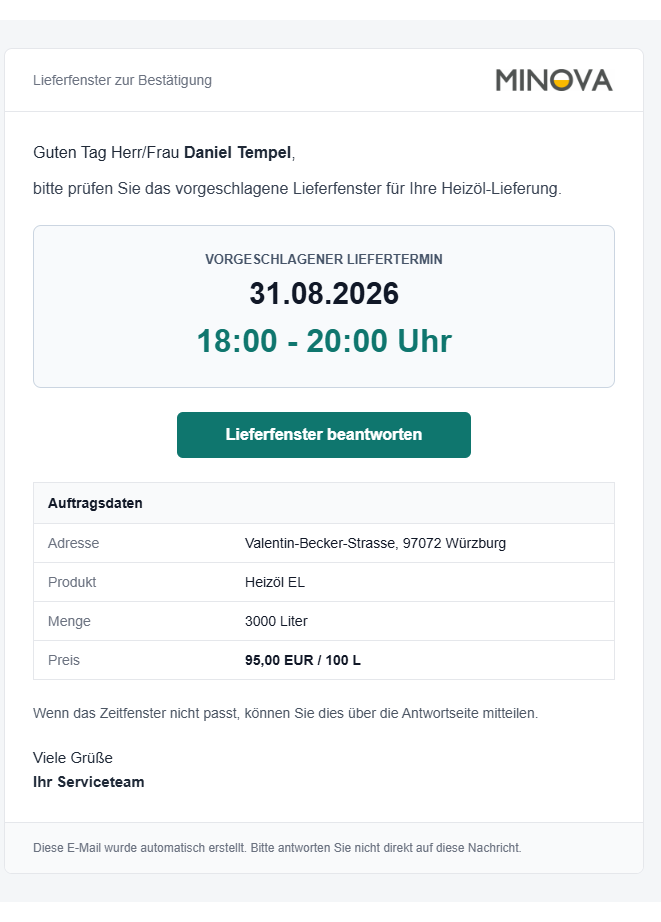
\includegraphics[
    width=0.82\textwidth,
    height=0.70\textheight,
    keepaspectratio
  ]{figures/rueckbestaetigungs-email.png}
  \caption{Beispiel einer durch den Avisierungsservice erzeugten
  Rückbestätigungs-E-Mail}
  \label{fig:rueckbestaetigungs-email}
  \par\smallskip
  {\footnotesize\textit{Quelle: Eigene Darstellung.}}
\end{figure}

Da SMTP-Infrastruktur und Absenderidentität mandantenbezogen konfigurierbar
sind, wird kein globaler Mail-Sender für alle Unternehmen verwendet. Für einen
konkreten Versand wird über den Auftrag die zugehörige \texttt{Company}
bestimmt und deren SMTP-Konfiguration geladen. Diese umfasst unter anderem
SMTP-Host und -Port, Sicherheitsmodus, optionale Authentifizierung sowie
Absenderadresse und Absendername. Die Einstellungen werden somit
mandantenbezogen gespeichert und nicht als globale Anwendungskonfiguration
geführt.

Auf Grundlage dieser Einstellungen wird zur Laufzeit ein Mail-Sender für den
jeweiligen Mandanten konfiguriert. Unterstützt werden die Sicherheitsmodi
\texttt{STARTTLS}, \texttt{IMPLICIT\_TLS} und \texttt{NONE}. Bei aktivierter
SMTP-Authentifizierung werden zusätzlich Benutzername und Kennwort
berücksichtigt. Das gespeicherte Kennwort wird erst für den Aufbau der
Verbindung entschlüsselt; seine kryptografische Absicherung wird in
Abschnitt~\ref{sec:konfigurationsschutz} behandelt. Die dynamische
Konfiguration ermöglicht die Verwendung unterschiedlicher SMTP-Einstellungen
je Mandant, erfordert jedoch den erneuten Aufbau des Mail-Senders für den
jeweiligen Versand.

Anschließend werden der zuvor erzeugte HTML-Inhalt und die
mandantenspezifische SMTP-Konfiguration für den Versand zusammengeführt. Als
Absender dienen die hinterlegte Adresse und Bezeichnung des Mandanten, als
Empfänger die im Auftrag gespeicherte E-Mail-Adresse des Kunden. Die Nachricht
enthält Betreff, HTML-Inhalt und ein eingebettetes Logo und wird anschließend
an den konfigurierten SMTP-Server übergeben. Fehlt für den Mandanten eine
SMTP-Konfiguration, kann kein Versand erfolgen. Technische Fehler bei der
Vorbereitung oder Übertragung der Nachricht werden gegenüber der
Anwendungslogik über eine gemeinsame Versandfehlerabstraktion dargestellt.

Die SMTP-Einstellungen können mandantenbezogen gelesen und aktualisiert werden.
Ein gespeichertes Kennwort wird dabei nicht an den Client zurückgegeben;
stattdessen zeigt \texttt{passwordConfigured} lediglich an, ob ein Kennwort
vorhanden ist. Wird bei aktivierter Authentifizierung kein neues Kennwort
übermittelt, bleibt das bestehende erhalten. Dadurch können die übrigen
SMTP-Einstellungen geändert werden, ohne das gespeicherte Kennwort erneut
übertragen zu müssen.

Wird die SMTP-Authentifizierung deaktiviert, werden die dafür nicht mehr
benötigten Zugangsdaten aus der Konfiguration entfernt. Ein Betrieb ohne
Authentifizierung und ohne Transportverschlüsselung ist im Projekt jedoch
ausschließlich für die lokale Entwicklungsumgebung vorgesehen, in der mit
einem lokalen Mailserver gearbeitet wird. Für einen produktiven Einsatz ist
eine authentifizierte und transportgesicherte SMTP-Verbindung vorgesehen. Die
bereitgestellte Entwicklungsumgebung verwendet entsprechend einen lokalen
SMTP-Server ohne Authentifizierung.

Zur technischen Prüfung stehen ein Verbindungstest und ein separater
Testversand zur Verfügung. Der Verbindungstest verwendet dieselbe
mandantenspezifische Konfiguration wie der reguläre Versand und prüft, ob mit
den gespeicherten Verbindungs- und gegebenenfalls Authentifizierungsdaten eine
Verbindung zum SMTP-System hergestellt werden kann.

Der Testversand führt mit derselben Transportkonfiguration eine tatsächliche
SMTP-Sendeoperation aus und sendet eine einfache Testnachricht an die
konfigurierte Absenderadresse. Die fachliche Erzeugung einer
Rückbestätigungs-E-Mail mit Thymeleaf-Template, Auftragsdaten und
Bestätigungslink ist davon nicht umfasst. Ein erfolgreicher Testversand zeigt
daher lediglich, dass der SMTP-Server bei der Übertragung keinen Fehler
gemeldet hat; eine endgültige Zustellung in das Postfach des Empfängers wird
damit nicht nachgewiesen.

Die E-Mail-Implementierung verbindet somit eine getrennte HTML-Aufbereitung mit
einer zur Laufzeit bestimmten mandantenspezifischen SMTP-Konfiguration. Die in
Abschnitt~\ref{sec:sms-whatsapp} betrachteten Kanäle SMS und WhatsApp verwenden
dagegen eine externe Provider-Anbindung.

\subsubsection{SMS und WhatsApp über Twilio: Technologieauswahl und Integration}
\label{sec:sms-whatsapp}
% Zuständigkeit: anderes Teammitglied.
% TODO: Inhalt durch das zuständige Teammitglied ergänzen.
\contentplaceholder

\subsection{Mandantenfähigkeit und Sicherheitskonzept}
\label{sec:sicherheitskonzept}

Der Avisierungsservice ist als mandantenfähige gemeinsame Anwendung konzipiert.
Mehrere voneinander unabhängige Unternehmen nutzen dieselbe fachliche
Funktionalität und eine einheitlich definierte DISPO-Schnittstelle. Auftrags-
und Kundendaten sowie mandantenspezifische Konfigurationen müssen dabei
eindeutig einem Unternehmen zugeordnet und voneinander getrennt verarbeitet
werden.

Aus den unterschiedlichen Zugriffs- und Vertrauenskontexten ergeben sich mehrere
Schutzbereiche mit jeweils eigenen Zugriffsmodellen. Die Zuordnung dieser
Schutzbereiche zu den nachfolgenden Abschnitten ist in
Tabelle~\ref{tab:schutzbereiche} zusammengefasst.

\begin{table}[htbp]
  \centering
  \caption{Schutzbereiche des Mandanten- und Sicherheitskonzepts}
  \label{tab:schutzbereiche}
  \small
  \begin{tabularx}{\textwidth}{
      @{}
      >{\raggedright\arraybackslash}p{0.30\textwidth}
      >{\raggedright\arraybackslash}X
      >{\centering\arraybackslash}p{0.12\textwidth}
      @{}
    }
    \toprule
    Schutzbereich
      & Sicherheitsaufgabe
      & Abschnitt \\
    \midrule
    DISPO-Schnittstelle
      & externes System authentifizieren und Mandantenidentität bestimmen
      & \ref{sec:dispo-authentifizierung} \\
    Dashboard-Zugriff
      & Browserzugriff an einen authentifizierten Mandantenkontext binden
      & \ref{sec:dashboard-zugriff} \\
    Kundenzugriff
      & Zugriff auf eine konkrete Rückbestätigungsanfrage begrenzen
      & \ref{sec:kundenzugriff-token} \\
    Mandantenspezifische Konfigurationsgeheimnisse
      & sensible technische Konfigurationsdaten vertraulich speichern
      & \ref{sec:konfigurationsschutz} \\
    \bottomrule
  \end{tabularx}
\end{table}

Zunächst wird betrachtet, wie die Mandantenidentität innerhalb der Anwendung
repräsentiert und für die logische Trennung gemeinsam gespeicherter Daten
verwendet wird.

\subsubsection{Mandantenkontext und Datenisolation}
\label{sec:mandantenkontext}

Für die Datenhaltung wurde bewusst eine gemeinsame Datenbank mit gemeinsamem
Schema gewählt. Separate Datenbanken ermöglichen eine stärkere physische
Isolation, getrennte Schemas eine stärkere strukturelle Trennung. Beide
Varianten erhöhen jedoch den mandantenspezifischen Provisionierungs-,
Migrations- und Betriebsaufwand. Das realisierte Modell lässt sich als
Pool-Modell einordnen, bei dem mehrere Mandanten dieselben Speicherstrukturen
nutzen und ihre Daten logisch über eine Mandantenidentität getrennt werden
\parencite{aws2021partitioningModels}. Da für die
angebundenen Unternehmen dieselbe Fachlogik und Datenstruktur gelten, wurde für
den Projektumfang der geringere infrastrukturelle Aufwand gegenüber einer
stärkeren Isolation priorisiert.

Zur Laufzeit wird eine bereits bestimmte Mandantenidentität durch den
\texttt{CompanyContext} repräsentiert, der ausschließlich die interne
\texttt{companyId} enthält. Dadurch müssen die mandantenbezogenen
Anwendungsfälle der DISPO-, Dashboard- und Konfigurationsschnittstellen den
vorgelagerten Authentifizierungsmechanismus nicht kennen. Die
Mandantenidentität wird nicht aus frei übermittelbaren fachlichen Request-Daten
übernommen, sondern zuvor durch den jeweiligen Sicherheitsmechanismus bestimmt
und anschließend getrennt von den Nutzdaten an die Anwendungslogik übergeben.
Die konkrete Ermittlung des \texttt{CompanyContext} für die DISPO-Schnittstelle
wird in Abschnitt~\ref{sec:dispo-authentifizierung} erläutert.

Der \texttt{CompanyContext} erzeugt für sich genommen noch keine
Datenisolation. Entscheidend ist seine Verwendung bei den nachfolgenden
Datenzugriffen. So wird ein bestehender DISPO-Auftrag anhand der Kombination aus
\texttt{companyId} und externer Auftrags-ID gesucht. Dadurch kann dieselbe
externe Auftrags-ID bei verschiedenen Unternehmen vorkommen, während sie
innerhalb eines Mandanten eindeutig bleibt.

Auch Dashboard-Abfragen werden auf die im \texttt{CompanyContext} enthaltene
\texttt{companyId} eingeschränkt. Die Detailansicht bestimmt zunächst den
Auftrag im Kontext des Mandanten und lädt anschließend die zugehörigen
Rückbestätigungsanfragen und Kundenreaktionen. Mandantenspezifische technische
Konfigurationen folgen demselben Prinzip; beispielsweise werden die in
Abschnitt~\ref{sec:emailversand} beschriebenen SMTP-Einstellungen über die
zugehörige \texttt{Company} bestimmt.

Datenbankseitige Fremdschlüssel- und Eindeutigkeitsbedingungen stellen die
konsistente Zuordnung von Datensätzen zu einer \texttt{Company} sicher,
ersetzen jedoch keine Zugriffsbeschränkung. Eine fehlerhaft formulierte Abfrage
könnte trotz korrekter Datenzuordnung Datensätze eines anderen Mandanten
berücksichtigen. Mandantentrennung ist daher von der bloßen Authentifizierung
zu unterscheiden: Auch ein authentifizierter Zugriff muss auf die Ressourcen
des zugehörigen Mandanten beschränkt werden
\parencite{aws2022tenantIsolation}.

Nicht alle Verarbeitungspfade verwenden den \texttt{CompanyContext}. Interne
Workflow-Schritte arbeiten mit bereits persistierten technischen
Objektidentifikatoren und den darüber erreichbaren fachlichen Beziehungen. Der
Kundenzugriff verwendet dagegen einen begrenzten tokenbasierten Zugriff auf
eine konkrete Rückbestätigungsanfrage, der in
Abschnitt~\ref{sec:kundenzugriff-token} behandelt wird.

Eine zusätzliche datenbankseitige Zugriffskontrolle durch Row-Level Security
oder einen globalen ORM-Tenant-Filter wird nicht eingesetzt; neue
mandantenbezogene Datenzugriffe müssen den jeweiligen Mandantenbezug daher
explizit berücksichtigen.

Ein Laufzeit-Onboarding neuer Mandanten ist im aktuellen Prototyp nicht
umgesetzt. Der initiale \texttt{Company}-Datensatz wird über die
Datenbankmigration bereitgestellt; ein festgelegter Anwendungsprozess zur
Aufnahme weiterer Mandanten besteht nicht. Das Datenmodell selbst ist jedoch
nicht auf einen einzelnen Mandanten beschränkt.

Die Mandantentrennung entsteht somit durch das Zusammenspiel aus einer
vertrauenswürdig bestimmten Mandantenidentität, ihrer Weitergabe als
\texttt{CompanyContext}, mandantenbezogenen Datenzugriffen und
datenbankseitiger Zuordnungsintegrität. Wie die Mandantenidentität bei einem
Zugriff durch DISPO ermittelt wird, beschreibt der folgende Abschnitt.

\subsubsection{Authentifizierung der DISPO-Schnittstelle}
\label{sec:dispo-authentifizierung}

Für die System-zu-System-Kommunikation wurde eine mandantenspezifische
API-Key-Authentifizierung gewählt. Sie ermöglicht die direkte Zuordnung des
aufrufenden externen Systems DISPO zu einer \texttt{Company}, ohne zusätzliche
Identity-Provider-Infrastruktur zu benötigen. Die Pfade unter
\texttt{/api/dispo/**} bilden hierfür einen eigenen zustandslosen Schutzbereich.
Der API-Key wird bei jeder HTTP-Anfrage im Header
\texttt{X-API-Key} übermittelt und erneut geprüft. Dem vergleichsweise geringen
Integrationsaufwand steht die Verwendung eines wiederverwendbaren Secrets
gegenüber, dessen Schutz und Lebenszyklus gesondert berücksichtigt werden
müssen.

Zur Authentifizierung wird der empfangene API-Key mit SHA-256 gehasht und der
resultierende Wert mit den gespeicherten API-Key-Hashes der
\texttt{Company}-Datensätze abgeglichen. Bei erfolgreicher Zuordnung wird aus
der internen \texttt{Company.id} ein \texttt{CompanyContext} erzeugt und als
Principal des authentifizierten Aufrufs verwendet. Die fachliche Verarbeitung
erhält damit ausschließlich den bestimmten Mandantenkontext und nicht den
Rohschlüssel. Fehlt der API-Key oder kann sein Hash keiner \texttt{Company}
zugeordnet werden, wird die Anfrage vor der fachlichen Verarbeitung mit
\texttt{401 Unauthorized} zurückgewiesen.

Der API-Key wird nicht im Klartext in der Anwendungsdatenbank persistiert;
jeder \texttt{Company} ist ein eindeutiger \texttt{apiKeyHash} zugeordnet. Eine
Offenlegung der Datenbank legt den Rohschlüssel dadurch nicht unmittelbar
offen. Da der verwendete SHA-256-Hash jedoch eine Offline-Prüfung möglicher
Schlüsselwerte erlaubt, müssen die API-Keys kryptografisch zufällig und mit
ausreichender Entropie erzeugt werden
\parencite{owaspSecretsManagement}.

Die Verwaltung des Schlüssellebenszyklus erfolgt im aktuellen Prototyp
außerhalb der Anwendung. Eine Änderung oder ein Widerruf erfordert den
administrativen Austausch des gespeicherten Hashwertes; automatische Rotation,
Ablaufzeiten oder die parallele Gültigkeit mehrerer Schlüssel sind nicht
implementiert.

Von der Authentifizierung ist die anschließende Autorisierung zu unterscheiden.
Ein gültiger API-Key authentifiziert die zugeordnete \texttt{Company}. Die
aktuelle Autorisierungsregel gewährt jedem so authentifizierten Principal
Zugriff auf sämtliche Endpunkte unter \texttt{/api/dispo/**}. Eine weitere
Differenzierung nach Rollen, Scopes oder endpointbezogenen Berechtigungen ist
nicht implementiert. Damit besteht eine technische Identität pro
\texttt{Company} mit einheitlichem Berechtigungsumfang.

Die beschriebene Authentifizierung betrifft ausschließlich eingehende
DISPO-Aufrufe. Die in Abschnitt~\ref{sec:statusrueckmeldung-dispo} beschriebene
ausgehende Statusrückmeldung enthält im aktuellen Prototyp keinen zusätzlichen
anwendungsseitigen Authentifizierungsnachweis. Der darauf aufbauende
Browserzugriff auf das Avisierungsdashboard verwendet einen separaten
Sicherheitsmechanismus, der im folgenden Abschnitt behandelt wird.

\subsubsection{Zugriffsschutz des Avisierungsdashboards}
\label{sec:dashboard-zugriff}

Der Zugriff auf das Avisierungsdashboard bildet einen anderen Schutzbereich
als die in Abschnitt~\ref{sec:dispo-authentifizierung} beschriebene
System-zu-System-Kommunikation. Als Vertrauensannahme gilt, dass DISPO den
jeweiligen Disponenten bereits authentifiziert hat. Der
Avisierungsservice überprüft diese personenbezogene Identität nicht selbst,
sondern bestimmt über die authentifizierte DISPO-Schnittstelle ausschließlich
den zugehörigen Mandanten. Der DISPO-API-Key verbleibt innerhalb der
System-zu-System-Kommunikation und wird nicht an den Browser weitergegeben. Für
den Dashboardzugriff wird somit die bereits bestimmte Mandantenidentität
übertragen, nicht das langfristig gültige Authentifizierungsgeheimnis.

Fordert DISPO einen Dashboardzugriff an, erzeugt der Avisierungsservice einen
kurzlebigen Einmalcode für die im \texttt{CompanyContext} enthaltene
\texttt{companyId}. Der Code basiert auf 32 kryptografisch zufälligen Bytes,
wird serverseitig der Mandantenidentität zugeordnet und ist eine Minute gültig.
DISPO erhält eine Frontend-URL mit dem Code als Query-Parameter und öffnet diese
im vorgesehenen Integrationsablauf im Browser des Disponenten. Der
Avisierungsservice selbst führt keine HTTP-Weiterleitung aus.

Der Besitz eines gültigen Codes berechtigt einmalig zum Aufbau einer
Dashboard-Sitzung für den zugeordneten Mandanten; eine Bindung an einen
bestimmten Browser oder Disponenten besteht nicht. Bis zu seiner Verwendung
stellt der Code daher einen kurzlebigen, besitzgebundenen Berechtigungsnachweis
dar. Da er über einen URL-Parameter übertragen wird, kann er beispielsweise in
der Browserhistorie oder in Protokolldaten sichtbar werden. Die kurze Gültigkeit
und die einmalige Verwendbarkeit begrenzen dieses Risiko, beseitigen es jedoch
nicht vollständig.

Das Avisierungsdashboard übermittelt den Code anschließend an den
Exchange-Endpunkt des Avisierungsservice. Beim Austausch wird der Eintrag aus
dem In-Memory-Speicher entfernt und seine zeitliche Gültigkeit geprüft. Aus der
gespeicherten Mandantenzuordnung wird ein \texttt{CompanyContext}
wiederhergestellt, als
authentifizierter Principal in den Spring-Security-Kontext übernommen und in
einer serverseitigen HTTP-Sitzung gespeichert. Für die Authentifizierung
weiterer Dashboardzugriffe verwendet der Browser ausschließlich die vom
Avisierungsservice ausgestellte Session-ID im Cookie; bei zustandsändernden
Anfragen kommt zusätzlich ein CSRF-Token zum Einsatz.

Das Session-Cookie ist mit \texttt{HttpOnly} und \texttt{SameSite=Lax}
konfiguriert; im Produktivprofil wird zusätzlich \texttt{Secure} verwendet.
\texttt{SameSite=Lax} begrenzt die automatische Übermittlung des Cookies in
bestimmten siteübergreifenden Kontexten, ersetzt jedoch keinen eigenständigen
CSRF-Schutz. Besteht bereits eine HTTP-Sitzung, wird deren Kennung beim Aufbau
der Authentifizierung erneuert, um die Übernahme einer zuvor bekannten
Sitzungskennung zu vermeiden. Dies dient dem Schutz vor
Session-Fixation-Angriffen.

Für die Sitzung ist eine Inaktivitätsdauer von acht Stunden konfiguriert. Sie
beschreibt keine absolute maximale Lebensdauer; die Sitzung wird ungültig, wenn
innerhalb dieses Zeitraums keine ihr zugeordnete Anfrage eingeht. Eine
zusätzliche absolute Laufzeitbegrenzung ist im Prototyp nicht vorgesehen.

Mit Ausnahme des Exchange-Endpunkts erfordern die Pfade unter
\texttt{/api/dashboard/**} einen authentifizierten Security Context. Der darin
gespeicherte \texttt{CompanyContext} wird den Dashboard-Anwendungsfällen als
Mandantenkontext übergeben. Die Mandantenidentität wird somit nicht aus
Request-Parametern oder fachlichen Nutzdaten bestimmt; die weitere
Datenisolation erfolgt wie in Abschnitt~\ref{sec:mandantenkontext} beschrieben.

Da der Browser das Session-Cookie automatisch mitsendet, werden
zustandsändernde Dashboardzugriffe zusätzlich durch CSRF-Schutz abgesichert.
Nach dem Sitzungsaufbau kann ein CSRF-Token abgerufen und im Header
\texttt{X-CSRF-TOKEN} übertragen werden. Im gewählten Ablauf wird vor dem
Austausch des Einmalcodes keine vorbereitende Dashboard-Sitzung mit CSRF-Token
aufgebaut; der Exchange-Endpunkt ist daher in der aktuellen Implementierung
vom regulären CSRF-Schutz ausgenommen. Der Einmalcode begrenzt diesen initialen
Zugriff zeitlich und auf eine einmalige Verwendung, stellt jedoch keinen
allgemeinen Schutz gegen Login-CSRF dar
\parencite{owaspCsrfPrevention}.

Ergänzend erlaubt die CORS-Konfiguration die Nutzung der
Dashboard-Schnittstelle unter Einbeziehung von Cookies ausschließlich für die
konfigurierte Frontend-Adresse und den benötigten CSRF-Header. CORS ersetzt
dabei weder die Authentifizierung noch den CSRF-Schutz.

Abbildung~\ref{fig:dashboard-sitzung} fasst den Übergang vom authentifizierten
DISPO-Kontext zur browserbasierten Dashboard-Sitzung zusammen.

\begin{figure}[htbp]
  \centering
  \begin{tikzpicture}[
      x=1cm,
      y=0.68cm,
      participant/.style={font=\small\sffamily\bfseries},
      lifeline/.style={densely dashed, draw=black!60, line width=0.45pt},
      message/.style={
        -{Latex[length=2.1mm,width=1.5mm]},
        draw=black!85,
        line width=0.65pt
      },
      msglabel/.style={
        font=\footnotesize\sffamily,
        align=left,
        fill=black!3,
        inner xsep=2pt,
        inner ysep=1pt
      },
      internal/.style={
        font=\footnotesize\sffamily,
        align=left,
        anchor=west
      }
    ]
    \filldraw[
      fill=black!3,
      draw=black!25,
      rounded corners=3pt
    ] (-0.9,0.55) rectangle (12.9,-15.3);

    \node[participant] at (0,0) {DISPO};
    \node[participant] at (6,0) {Avisierungsservice};
    \node[participant] at (12,0) {Browser};

    \draw[lifeline] (0,-0.35) -- (0,-14.8);
    \draw[lifeline] (6,-0.35) -- (6,-14.8);
    \draw[lifeline] (12,-0.35) -- (12,-14.8);

    \draw[message] (0,-1.4) --
      node[midway,above,msglabel] {Dashboardzugriff\\+ \texttt{X-API-Key}}
      (6,-1.4);

    \node[internal] at (6.2,-2.35) {Einmalcode erzeugen};

    \draw[message] (6,-3.3) --
      node[midway,above,msglabel] {Frontend-URL + Code}
      (0,-3.3);

    \draw[message] (0,-4.7) --
      node[midway,above,msglabel] {URL öffnen}
      (12,-4.7);

    \draw[message] (12,-6.0) --
      node[midway,above,msglabel] {Code austauschen}
      (6,-6.0);

    \node[internal] at (6.2,-6.95) {
      \texttt{CompanyContext} in Session\\speichern
    };

    \draw[message] (6,-8.2) --
      node[midway,above,msglabel] {Session-Cookie}
      (12,-8.2);

    \draw[message] (12,-9.9) --
      node[midway,above,msglabel] {
        \texttt{GET /api/dashboard/csrf}\\+ Session-Cookie
      }
      (6,-9.9);

    \draw[message] (6,-11.4) --
      node[midway,above,msglabel] {CSRF-Token}
      (12,-11.4);

    \draw[message] (12,-13.6) --
      node[midway,above,msglabel] {
        Zustandsändernde Anfrage\\
        + Session-Cookie\\
        + \texttt{X-CSRF-TOKEN}
      }
      (6,-13.6);
  \end{tikzpicture}
  \caption{Übergang vom authentifizierten DISPO-Kontext zur Dashboard-Sitzung}
  \label{fig:dashboard-sitzung}
\end{figure}

Das Sicherheitsmodell besitzt bewusst akzeptierte Grenzen. Der
Avisierungsservice authentifiziert ausschließlich die \texttt{Company}, nicht
den einzelnen Disponenten; eigene Benutzerkonten, Rollen und personenbezogene
Berechtigungen bestehen daher nicht. Die Einmalcodes werden nur im lokalen
Arbeitsspeicher gespeichert, weshalb der Mechanismus auf eine einzelne Instanz
des Avisierungsservice ausgelegt ist. Auch die serverseitige Sitzung macht den
Betrieb zustandsbehaftet. Eine explizite Abmeldung wurde im Prototyp nicht
umgesetzt; ungenutzte Sitzungen verlieren nach Ablauf der konfigurierten
Inaktivitätsdauer ihre Gültigkeit.

Der davon getrennte Kundenzugriff wird im folgenden Abschnitt betrachtet.

\subsubsection{Tokenbasierter Kundenzugriff}
\label{sec:kundenzugriff-token}

Der Kundenzugriff bildet einen eigenen Schutzbereich. Im Unterschied zur
DISPO-Schnittstelle und zum Avisierungsdashboard verfügt der Kunde über keine
eigene technische Identität innerhalb des Avisierungsservice. Es existieren
weder Kundenkonten noch eine browserbasierte
Sitzung oder ein \texttt{CompanyContext}. Der Zugriff auf die kundenbezogenen
Funktionen erfolgt daher über einen zufällig erzeugten Zugriffstoken. Dieser
authentifiziert keine Person, sondern ermöglicht dem Besitzer den Zugriff auf
den damit verbundenen Kundenvorgang. Dadurch kann auf eine zusätzliche
Registrierung oder Anmeldung des Kunden verzichtet werden; gleichzeitig muss
der Token selbst vor unbefugter Weitergabe geschützt werden.

Bei der Neuanlage einer \texttt{ConfirmationRequest} wird ein neuer Token
erzeugt. Hierzu werden mit \texttt{SecureRandom} 32 zufällige Bytes generiert
und URL-kompatibel über \texttt{Base64} kodiert. Der daraus resultierende
Zufallswert besitzt 256 Bit Entropie und erschwert das Erraten gültiger Tokens.
Werden für einen Auftrag nacheinander mehrere Rückbestätigungsanfragen erzeugt,
erhält jede neu angelegte Anfrage einen eigenen Token.

Der Token wird Bestandteil des individuellen Bestätigungslinks und über die in
Abschnitt~\ref{sec:kundenkommunikation} beschriebenen Kommunikationskanäle an
den Kunden übertragen. Über denselben Token kann anschließend die
Bestätigungsseite aufgerufen, eine Kundenreaktion übermittelt und auf die für den
Kunden vorgesehenen Funktionen der Lieferverfolgung zugegriffen werden. Die
Zugriffsprüfung erfolgt
anhand des bei jedem Aufruf übermittelten Tokens. Da dabei keine authentifizierte
Browser-Sitzung verwendet wird, sind diese Endpunkte in der
Spring-Security-Konfiguration von der CSRF-Prüfung ausgenommen.

Für die Auflösung eines Tokens reicht dessen Existenz in der Datenbank nicht
aus. Er muss zusätzlich zur neuesten \texttt{ConfirmationRequest} des
jeweiligen Auftrags gehören. Technisch wird dafür geprüft, ob die zugehörige
Anfrage den höchsten Datenbankidentifikator unter den Rückbestätigungsanfragen
desselben Auftrags besitzt. Wird nach einer Anfrage A eine neuere Anfrage B
erzeugt, bleibt Token A zwar historisch gespeichert, kann über die
Kundenschnittstelle jedoch nicht mehr aufgelöst werden. Dadurch verlieren
ältere Kundenlinks ihre Gültigkeit, ohne dass die zugehörigen historischen
Anfragen gelöscht werden müssen.

Welche Funktion nach erfolgreicher Tokenauflösung genutzt werden kann, hängt
zusätzlich vom Zustand des Vorgangs ab. Die Bestätigungsseite bleibt auch
nach Ablauf der Antwortfrist verfügbar, solange keine neuere
Rückbestätigungsanfrage angelegt wurde. Dies ist bewusst vorgesehen, damit der
Kunde den Liefertermin später erneut einsehen und denselben Link am Liefertag
für die Funktionen der Lieferverfolgung verwenden kann. Eine nachträgliche
Bestätigung oder Ablehnung ist dagegen nicht möglich, da hierfür zusätzlich
geprüft wird, ob die Anfrage noch aktiv, nicht abgelaufen und noch unbeantwortet
ist.

Auch die Funktionen der Lieferverfolgung verwenden dieselbe Tokenauflösung.
Informationen zur Lieferverfolgung werden nur an dem im
\texttt{DeliverySlot} hinterlegten Lieferdatum als verfügbar ausgewiesen. Eine
Fahrerposition wird zusätzlich nur dann bereitgestellt, wenn entsprechende
Positionsdaten vorliegen. Die funktionale Ermittlung dieser Daten wird in
Abschnitt~\ref{sec:lieferverfolgung} behandelt.

Der gewählte Zugriff über einen zufälligen Token besitzt dennoch Grenzen. Da
keine Personenidentität überprüft wird, kann grundsätzlich jeder, der einen
aktuellen Token erhält, die dafür freigegebenen Funktionen verwenden. Im
aktuellen Prototyp wird der Token zudem direkt in der Datenbank gespeichert;
eine hashbasierte Speicherung wäre als zusätzliche Härtungsmaßnahme möglich.

Die bewusst beibehaltene Lesbarkeit der Bestätigungsseite verlängert
außerdem den Zeitraum, in dem der jeweils letzte Token verwendbar bleibt.
Solange keine neuere \texttt{ConfirmationRequest} entsteht, kann die
Bestätigungsseite auch nach Antwortfrist und Liefertag weiterhin geöffnet
werden. Dies ermöglicht die spätere Einsicht in Lieferinformationen, erhöht
jedoch zugleich die Auswirkungen einer möglichen Offenlegung des Tokens.

Da der Token Bestandteil des URL-Pfades ist, kann eine Offenlegung
beispielsweise über Browserhistorien, URL-Protokollierung oder
Referer-Informationen erfolgen. Für den produktiven Betrieb wird daher eine
durchgängige HTTPS-Übertragung vorausgesetzt. Diese schützt die Übertragung,
verhindert jedoch nicht die spätere Offenlegung einer bereits bekannten oder
protokollierten URL \parencite{owaspInformationExposureUrls}.

Das Verfahren ermöglicht damit einen einfachen Kundenzugriff ohne zusätzliche
Benutzerverwaltung. Die zufällige Token-Erzeugung und die Prüfung auf die
jeweils neueste Rückbestätigungsanfrage erschweren das Erraten gültiger Tokens
und schließen veraltete Links aus. Der Schutz des aktuell gültigen Tokens
bleibt jedoch eine zentrale Voraussetzung des Zugriffsmodells.

\subsubsection{Schutz sensibler Konfigurationsdaten}
\label{sec:konfigurationsschutz}

Das mandantenspezifische SMTP-Kennwort stellt ein wiederverwendbares
technisches Zugangsgeheimnis dar. Da der Avisierungsservice den ursprünglichen
Wert später selbst zur Authentifizierung gegenüber dem SMTP-System benötigt,
reicht eine ausschließlich hashbasierte Speicherung, wie beim DISPO-API-Key,
nicht aus. Die reversible Verschlüsselung ergibt sich somit aus dem konkreten
technischen Verwendungszweck und ist keine Alternative zum Hashing von
Benutzerpasswörtern.

Zur vertraulichen Speicherung und Erkennung nachträglicher Veränderungen wird
AES-GCM mit einem 256-Bit-Schlüssel eingesetzt
\parencite{dworkin2007gcm,nist2023aes}. Für jeden Verschlüsselungsvorgang wird
ein neuer zufälliger
Initialisierungsvektor erzeugt. Zusätzlich wird die interne
\texttt{companyId} als Additional Authenticated Data einbezogen. Dadurch ist
das Chiffrat kryptografisch an den vorgesehenen Mandantenkontext gebunden; eine
Veränderung des Chiffrats oder dieses Kontexts führt bei der Entschlüsselung zu
einer fehlgeschlagenen Authentizitätsprüfung. Diese Bindung ergänzt die
mandantenbezogene Zugriffskontrolle aus
Abschnitt~\ref{sec:mandantenkontext}, ersetzt sie jedoch nicht.

Der verschlüsselte Passwortwert wird in der Anwendungsdatenbank gespeichert,
während der Master-Key über die externe Spring-Konfiguration bereitgestellt
wird. Schlüsselmaterial und Chiffrat sind damit logisch getrennt, sodass ein
isolierter Zugriff auf die Datenbank das SMTP-Kennwort nicht unmittelbar
offenlegt. Eine anwendungsseitige Integration eines externen Schlüssel- oder
Secrets-Management-Systems ist im Prototyp nicht umgesetzt.

Ein neu konfiguriertes Kennwort wird über die mandantengebundene
Konfigurationsschnittstelle übermittelt und vor der Persistierung
verschlüsselt. Für einen produktiven Betrieb setzt dieser Übertragungsweg eine
transportgesicherte HTTPS-Verbindung voraus. Bereits gespeicherte Kennwörter
werden, wie in Abschnitt~\ref{sec:emailversand} beschrieben, nicht erneut an
den Client ausgegeben. Zur technischen SMTP-Nutzung wird das Kennwort beim
Erzeugen des mandantenspezifischen Mail-Senders entschlüsselt, etwa für
regulären Versand, Verbindungstest oder Testversand. Der Klartextwert muss
daher zur Laufzeit innerhalb der Anwendung verarbeitet werden.

Die Lösung reduziert insbesondere das Risiko einer Offenlegung der
SMTP-Zugangsdaten bei einem isolierten Zugriff auf die Datenbank. Da sämtliche
mandantenspezifischen SMTP-Kennwörter denselben zentralen Master-Key verwenden,
kann dessen Kompromittierung potenziell sämtliche damit geschützten
Zugangsdaten betreffen; auch gegenüber einer vollständigen Kontrolle des
laufenden Anwendungsprozesses bietet die Verschlüsselung keinen Schutz. Eine
anwendungsseitige Schlüsselrotation ist im Prototyp ebenfalls nicht umgesetzt:
Das Chiffrat enthält zwar eine Formatversion, jedoch keinen Bezeichner des
verwendeten Master-Keys, und mehrere gleichzeitig gültige Schlüssel oder eine
automatische Neuverschlüsselung bestehender Werte werden nicht unterstützt.
Ein bloßer Austausch des Master-Keys führt deshalb dazu, dass bereits
gespeicherte Kennwörter nicht mehr entschlüsselt werden können.

\subsection{Abfragemodell für das Avisierungsdashboard}
\label{sec:abfragemodell}

Die in den vorhergehenden Abschnitten erzeugten Auftrags-, Avisierungs- und
Rückbestätigungsdaten müssen der Disposition für die operative Bearbeitung
bereitgestellt werden. Dazu bereitet der Avisierungsservice die gespeicherten
Fach- und Prozessdaten entsprechend dem jeweiligen Informationsbedarf auf.

Das in Abschnitt~\ref{sec:domaenenmodell} beschriebene
Domänenmodell bildet die fachlichen Beziehungen und Zustände von
\texttt{Order}, \texttt{ConfirmationRequest} und \texttt{CustomerResponse}
ab. Für die dispositionsseitige Darstellung werden diese Daten jedoch anders
strukturiert. Die persistierten Domänenobjekte werden daher nicht unmittelbar
ausgegeben; stattdessen werden die für den jeweiligen Anwendungsfall
benötigten Informationen gezielt zusammengestellt.

Das Abfragemodell unterscheidet hierzu zwei Sichten. Die Tourübersicht fasst
die für die operative Bearbeitung relevanten Informationen mehrerer Aufträge
im Kontext ihrer Touren zusammen und stellt dabei jeweils den aktuell
maßgeblichen Avisierungsstand dar. Die auftragsbezogene Detailansicht stellt
dagegen einen einzelnen Auftrag einschließlich seiner aktuellen und früheren
Avisierungen bereit. Beide Sichten greifen damit auf dieselben gespeicherten
Fach- und Prozessdaten zurück, unterscheiden sich jedoch in Umfang und Struktur
der bereitgestellten Informationen.

Eine separate Lesedatenhaltung wird hierfür nicht verwendet. Die benötigten
Ergebnisstrukturen werden bei der jeweiligen Abfrage aus derselben relationalen
Datenbasis erzeugt, die auch der schreibenden Verarbeitung zugrunde liegt. Im
Folgenden werden zunächst die Tourübersicht mit dynamischer Filterung,
Gruppierung und Paginierung und anschließend die auftragsbezogene Detailansicht
mit Avisierungshistorie betrachtet.

\subsubsection{Tourübersicht, dynamische Filterung, Gruppierung und Paginierung}
\label{sec:touruebersicht}

Die Tourübersicht stellt die für die operative Bearbeitung relevanten
Auftrags- und Avisierungsinformationen in einer tourbezogenen Struktur bereit.
Eine Tour enthält dabei ihre tourbezogenen Angaben sowie eine reduzierte Sicht
auf die zugehörigen Aufträge.

Da zu einem \texttt{Order} mehrere \texttt{ConfirmationRequest}-Objekte
existieren können, berücksichtigt die Übersicht je Auftrag ausschließlich die
Anfrage mit der höchsten internen ID. Frühere Rückbestätigungsanfragen bleiben
für die Avisierungshistorie erhalten, werden jedoch nicht zusätzlich in der
aktuellen Tourübersicht dargestellt.

Jede Abfrage wird zunächst auf die \texttt{companyId} des aktuellen Mandanten
eingeschränkt. Zusätzlich können Tournummern, fachliche
\texttt{ConfirmationStatus}, ein Datumsbereich und eine Freitextsuche
miteinander kombiniert werden. Der Statusfilter bezieht sich auf den
fachlichen Bearbeitungsstand des Auftrags und nicht auf den technischen
Versandstatus einer einzelnen Rückbestätigungsanfrage. Wird kein Startdatum
angegeben, dient das aktuelle Datum als Untergrenze; ungültige Datumsbereiche
werden zurückgewiesen. Die Freitextsuche berücksichtigt ohne Unterscheidung
von Groß- und Kleinschreibung Tournummer, Fahrzeugkennzeichen, externe
Auftrags-ID, Kundenname und Lieferadresse.

Für die dynamische Abfragekonstruktion wird QueryDSL in seiner JPA-Integration
eingesetzt. Die Bibliothek ermöglicht den typisierten Aufbau und die
schrittweise Zusammensetzung von Abfragebedingungen
\parencite{querydslUnifiedQueries}. Dadurch können nur die tatsächlich gesetzten
Filter berücksichtigt und mit der Auswahl der jeweils neuesten
Rückbestätigungsanfrage, Gruppierung, Sortierung und Paginierung kombiniert
werden. Separate statische Abfragen für jede mögliche Filterkombination sind
dadurch nicht erforderlich.

Da die Tour die zentrale Einheit der Übersicht bildet, erfolgt auch die
Paginierung auf Tour-Ebene und nicht auf einzelnen Aufträgen. Zunächst werden
daher die Touren der angeforderten Seite bestimmt und ihre Gesamtzahl für die
Paginierung ermittelt. Anschließend werden die zu diesen Touren gehörenden
Auftragsinformationen geladen. Dadurch beeinflusst die unterschiedliche Anzahl
von Aufträgen innerhalb einer Tour nicht die Einteilung der Tourseiten.

Die Filterbedingungen werden sowohl bei der Auswahl der Touren als auch beim
Laden ihrer Aufträge berücksichtigt. Bei auftragsbezogenen Filtern enthält eine
zurückgegebene Tour daher nur diejenigen Aufträge, die die gewählten
Bedingungen erfüllen. Die Touren werden nach Lieferdatum und Tournummer
sortiert, die enthaltenen Aufträge nach Beginn und Ende des Lieferfensters
sowie nach externer Auftrags-ID.

Für die Filterauswahl wird ergänzend eine reduzierte Abfrage der im aktuellen
Mandanten- und Datumsbereich verfügbaren Tournummern bereitgestellt. Sie
verwendet dieselben grundlegenden Mandanten-, Datums- und
Aktualitätsbedingungen wie die Tourübersicht, beschränkt die Suchfunktion
jedoch auf die Tournummer. Während die Tourübersicht damit den aktuell
maßgeblichen Bearbeitungsstand darstellt, behandelt
Abschnitt~\ref{sec:auftragsdetails-avisierungshistorie} zusätzlich die
einzelnen Avisierungsversuche und deren Historie.

\subsubsection{Auftragsdetails und Avisierungshistorie}
\label{sec:auftragsdetails-avisierungshistorie}

Während die Tourübersicht mehrere Aufträge in reduzierter Form darstellt,
bündelt die Detailansicht die Informationen zu einem einzelnen Auftrag. Dieser
wird innerhalb des bestehenden Mandantenkontexts über \texttt{companyId} und
externe Auftrags-ID ermittelt. Angezeigt werden die aktuellen Auftragsdaten
einschließlich Kunden- und Kontaktdaten, Lieferadresse, Produkt-, Mengen- und
Preisangaben, Tourdaten sowie \texttt{ConfirmationStatus}.

Anschließend werden alle über die interne \texttt{Order}-ID zugeordneten
\texttt{ConfirmationRequest}-Objekte geladen. Eine vorhandene
\texttt{CustomerResponse} wird per \texttt{LEFT JOIN} zugeordnet, sodass auch
unbeantwortete, ausstehende oder fehlgeschlagene Anfragen Bestandteil des
Ergebnisses bleiben.

Die interne ID dient als technisches Ordnungsmerkmal, da kein gesonderter
Erzeugungszeitpunkt gespeichert wird. Die Anfrage mit der höchsten ID wird als
\texttt{currentRequest} ausgewiesen; die übrigen bilden in absteigender
ID-Reihenfolge die \texttt{previousRequests}. \texttt{currentRequest} bedeutet
dabei nicht, dass die Anfrage noch aktiv ist. Liegt keine
Rückbestätigungsanfrage vor, bleibt dieser Bestandteil leer. Eine separate
Paginierung der Historie ist im Prototyp nicht vorgesehen.

Der auftragsbezogene \texttt{ConfirmationStatus} ist vom Darstellungsstatus
einer einzelnen Rückbestätigungsanfrage zu unterscheiden. Für diese werden die
in Abschnitt~\ref{sec:domaenenmodell} getrennt beschriebenen Merkmale
\texttt{deliveryStatus}, \texttt{active} und eine gegebenenfalls vorhandene
Kundenreaktion zu einem ansichtsspezifischen Status verdichtet.

\begin{table}[htbp]
  \centering
  \small
  \renewcommand{\arraystretch}{1.15}
  \caption{Darstellungsstatus einzelner Rückbestätigungsanfragen}
  \label{tab:anfrage-darstellungsstatus}
  \begin{tabularx}{\textwidth}{@{}
    >{\raggedright\arraybackslash}X
    >{\raggedright\arraybackslash}p{0.19\textwidth}@{}}
    \toprule
    \textbf{Zustand der Rückbestätigungsanfrage}
      & \textbf{Darstellungsstatus} \\
    \midrule
    \texttt{deliveryStatus = PENDING}
      & \texttt{PENDING} \\
    \texttt{deliveryStatus = FAILED}
      & \texttt{FAILED} \\
    \texttt{deliveryStatus = SENT}, \texttt{active = true}, keine
      Kundenreaktion
      & \texttt{SENT} \\
    \texttt{deliveryStatus = SENT}, \texttt{responseType = CONFIRM}
      & \texttt{CONFIRMED} \\
    \texttt{deliveryStatus = SENT}, \texttt{responseType = REJECT}
      & \texttt{REJECTED} \\
    \texttt{deliveryStatus = SENT}, \texttt{active = false}, keine
      Kundenreaktion
      & \texttt{NO\_RESPONSE} \\
    \bottomrule
  \end{tabularx}
\end{table}

Dadurch muss das Avisierungsdashboard die getrennten Zustandsinformationen nicht
selbst kombinieren. Die Verdichtung bewahrt jedoch nicht immer die Ursache der
Deaktivierung. Sowohl eine nach Fristablauf deaktivierte als auch eine durch
eine neuere Avisierung abgelöste Anfrage wird ohne Kundenreaktion als
\texttt{NO\_RESPONSE} dargestellt, da keine separate Deaktivierungsursache
gespeichert wird.

Die Historisierung ist auf anfragespezifische Daten begrenzt.
Kommunikationskanal, Lieferfenster, Antwortfrist und technischer Versandstatus
sowie gegebenenfalls Versand- und Ablaufzeitpunkte und Kundenreaktionen bleiben
je \texttt{ConfirmationRequest} erhalten. Allgemeine Auftragsdaten werden
dagegen aus dem aktuellen \texttt{Order} gelesen.

Die Detailansicht verbindet damit aktuelle Auftragsdaten mit einer Historie der
Avisierungsversuche, stellt jedoch keine vollständige Versionierung des
Auftrags dar. Frühere Kunden-, Adress-, Produkt- oder Tourdaten können nach
einer Änderung nicht rekonstruiert werden.

\subsection{Lieferverfolgung und Geocoding}
\label{sec:lieferverfolgung}
% TODO: Einführung in Lieferverfolgung und Geocoding ergänzen.

\subsubsection{Daten zur Lieferverfolgung und Fahrerposition}
% TODO: Inhalt ergänzen.
\contentplaceholder

\subsubsection{Zielkoordinaten und Geocoding}
% TODO: Inhalt ergänzen.
\contentplaceholder

\subsubsection{Bereitstellung für die Bestätigungsseite}
% Zuständigkeit: anderes Teammitglied.
% TODO: Inhalt durch das zuständige Teammitglied ergänzen.
\contentplaceholder

\subsection{Technische Konfiguration und lokale Integrationsumgebung}
\label{sec:technische-konfiguration}

Die technische Konfiguration des Avisierungsservice ist auf drei
Spring-Konfigurationsdateien verteilt. \texttt{application.yaml} enthält die
gemeinsamen Einstellungen des Avisierungsservice, während
\texttt{application-dev.yml} die für die lokale Entwicklung benötigten
Abweichungen ergänzt. Dazu gehören insbesondere die lokale Datenbankanbindung,
zusätzliche Flyway-Ressourcen für Entwicklungsdaten sowie die Adressen der
lokal angebundenen Systeme. \texttt{application-prod.yml} enthält davon
abweichende Einstellungen für den vorgesehenen Produktivbetrieb,
beispielsweise für Datenbankzugang, Frontend-Adresse und Session-Cookie.
Laufzeitabhängige beziehungsweise sensible Werte wie der Master-Key und die
Twilio-Zugangsdaten werden nicht fest in der Anwendung hinterlegt, sondern
über Umgebungsvariablen bereitgestellt. Für die lokale Entwicklung kann
hierfür eine von der Versionsverwaltung ausgeschlossene \texttt{.env}-Datei
verwendet werden.

Für die lokale Ausführung wurden das Webfrontend und der Avisierungsservice
containerisiert und in die gemeinsame \texttt{docker-compose.yml} aufgenommen.
Der Container des Avisierungsservice wird mit dem Profil \texttt{dev} gestartet.
Gemeinsam mit dem Webfrontend werden PostgreSQL, Mailpit, pgAdmin und der
DISPO-Mock bereitgestellt. PostgreSQL stellt die Anwendungsdatenbank bereit,
Mailpit nimmt lokal versendete E-Mails entgegen und der DISPO-Mock bildet die im
Projekt benötigten DISPO-Schnittstellen für Callback und Lieferverfolgung nach.
pgAdmin dient ergänzend zur manuellen Einsicht in die Datenbank, ist für den
Betrieb des Avisierungsservice jedoch nicht erforderlich.

Die für den Containerbetrieb benötigten Adressen werden in Docker Compose an
die interne Umgebung angepasst. Der Avisierungsservice verwendet dadurch für
Datenbank, SMTP und DISPO die innerhalb des Compose-Netzwerks bereitgestellten
Dienste anstelle der für einen direkten lokalen Start vorgesehenen
\texttt{localhost}-Adressen. Für PostgreSQL wird vor dem Start des
Avisierungsservice zusätzlich ein erfolgreicher Healthcheck abgewartet. Das
\texttt{dev}-Profil ergänzt den regulären Flyway-Ablauf um ein
entwicklungsbezogenes Callback zur
Erzeugung lokaler Ausgangsdaten; die dafür benötigten SMTP- und DISPO-Adressen
werden über konfigurierbare Platzhalter bereitgestellt. Die eigentliche
Schemaentwicklung wurde bereits in Abschnitt~\ref{sec:persistenzmodell}
beschrieben.

Damit kann die für die Entwicklung der digitalen Lieferavisierung benötigte
Umgebung gemeinsam über Docker Compose bereitgestellt werden. Externe Dienste
wie Twilio und der Geocoding-Dienst bleiben außerhalb dieser lokalen Umgebung
und werden bei Bedarf direkt angebunden. Mailpit und der DISPO-Mock ersetzen
damit nur die für die Entwicklung benötigten Schnittstellen, nicht die
vollständigen Produktivsysteme.

\clearpage
\printbibliography[heading=bibintoc,title={Literaturverzeichnis}]

\end{document}
